\cleardoublepage

\addcontentsline{toc}{chapter}{\numberline{}Optimisation combinatoire et méthodes de résolutions }
\addtocontents{lof}{\textbf{Optimisation combinatoire et méthodes de résolutions }}

\setcounter{chapter}{2}
\setcounter{section}{0}
\setcounter{figure}{0}

\begin{center}
	\Huge\textbf{Optimisation combinatoire et méthodes de résolutions }
\end{center}

\section{Introduction}
L’optimisation combinatoire occupe une place très importante dans divers domaines. En effet, elle définit un cadre formel pour de nombreux problèmes dans plusieurs secteurs tels que l’industrie, la finance ou tout simplement les problèmes de la vie quotidienne.
La solution optimale à un problème d’optimisation ne peut que très rarement être déterminée en un temps polynomial. Il est donc souvent nécessaire de trouver des modes de résolution qui fournissent une solution de bonne qualité dans un laps de temps raisonnable. Il existe donc des méthodes de résolution exactes qui sont caractérisées par le fait qu’elles permettent d’obtenir une ou plusieurs solutions optimales, ainsi que des méthodes de résolution approchées qui fournissent des solutions de bonne qualité (proches de l’optimal mais sans garantie d’optimalité) et dont le temps de résolution sera plus faible \cite{zidi2006systeme}.

Ce chapitre sera structuré comme suit : d’abord, nous allons présenter brièvement les techniques de routage dans les RCSFs, par la suite nous nous pencherons sur les techniques d’optimisation combinatoire, exactes et approchées surtout, pour la résolution des problèmes NP-Difficiles. Tout ceci sera clôturé par une conclusion.

Depuis une vingtaine d’années, les heuristiques les plus populaires, et également les plus efficaces, sont des techniques générales, appelées méta-heuristiques, qu’il s’agit de l’adapter à chaque problème dont sa complexité est NP-hard. Dans ce chapitre, nous allons définir c’est quoi une méta-heuristique, la classification des méthodes utilisées dans les méta-heuristiques. 

\section{Techniques d’optimisation combinatoire:}
L’importance de l’optimisation combinatoire se justifie d’un coté par la grande difficulté des problèmes d’optimisation et d’un autre coté par la quantité innombrable d’applications pratiques pouvant être formulées sous la forme de tels problèmes. En effet, ces derniers sont souvent faciles à formaliser ou à exprimer, mais peuvent toutefois, être très difficiles à résoudre. Néanmoins, la plupart d’entre eux ne possèdent pas à ce jour de solution efficace valable pour toutes les données. \cite{hao1999metaheuristiques}

Un problème d’optimisation combinatoire est exprimé sous forme d’une fonction objectif qui est à maximiser, ou à minimiser, selon le type de problème traité. La résolution d’un tel problème revient à chercher la meilleure solution (optimum global) dans l’ensemble des solutions réalisables, sans pour autant être coincé dans des solutions intermédiaires (optimum locaux), propres à un sous-espace de recherche (voir Figure \ref{fig:DOGOL}).

\begin{figure}[H]
	\centering
	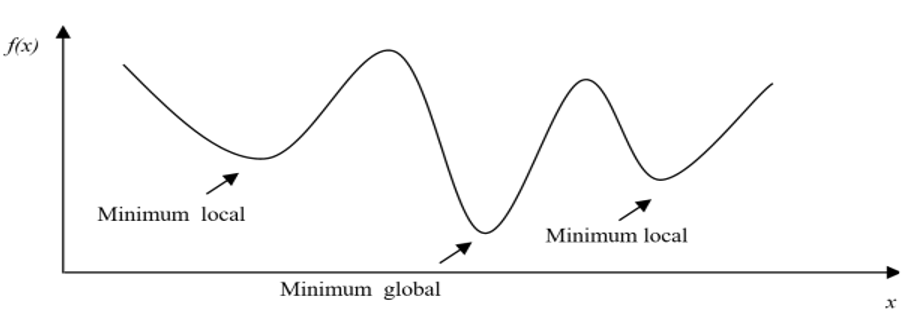
\includegraphics[width=15cm,height=5cm]{Chap2/1.png}
	\caption{Différence entre un optimum global et des optima locaux}
	\label{fig:DOGOL}
\end{figure}

L’élégance des problèmes d’optimisation combinatoire réside dans la possibilité de les modéliser en problèmes de la théorie des graphes et ainsi profiter des outils de cette dernière.

\begin{figure}[H]
	\centering
	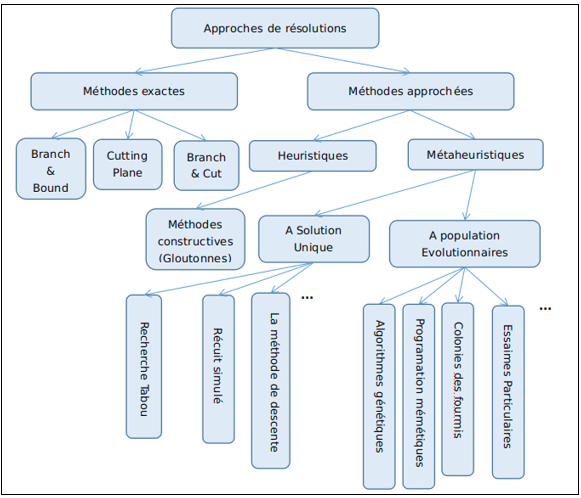
\includegraphics[width=15cm,height=13cm]{Chap2/2.png}
	\caption{Classification des méthodes de résolution d’optimisation combinatoire}
	\label{fig:CMROC}
\end{figure}

De nombreuses méthodes de résolution ont été développées par la communauté scientifique (recherche opérationnelle, intelligence artificielle).

Ces méthodes sont divisées en deux grandes catégories : les méthodes exactes basées sur l’énumération de toutes les solutions réalisables, chose qui garantie la complétude de la résolution, et les méthodes approchées qui perdent en exactitude pour gagner en efficacité \cite{park2007dominating} . La figure \ref{fig:CMROC} illustre un schéma résumant la classification des différentes méthodes discutées le long du chapitre.

\subsection{Méthodes exacte}
Ces méthodes sont dites complètes ou exactes car elles permettent de trouver la solution optimale pour une instance de taille finie dans un temps limité et de prouver son optimalité \cite{puchinger2005combining} . Ces méthodes se basent généralement sur sur une recherche complètes de l’espace des combinaisons afin de trouver une solution optimale.\\
Les algorithmes exacts les plus réussis dans la littérature: 


\begin{enumerate}[label=\alph*)]
	\item \textbf{La méthode séparation et évaluation (Branch and Bound):} elle repose sur une méthode arborescente de recherche d’une solution optimale par séparations et évaluations. Le branch-and-bound est basé sur trois axes principaux: L’évaluation, la séparation, la stratégie de parcours.
	\begin{itemize}
		\item \textbf{L’évaluation: } permet de réduire l’espace de recherche en éliminant quelques sous ensembles qui ne contiennent pas la solution optimale.
		\item \textbf{La séparation: } a pour but de choisir un sous-problème parmi tous ceux non encore choisis. Elle associe donc à chacun une évaluation (valeur minimale) de toutes les solutions le constituant. Un sous-problème peut être supprimé dans le cas où son évaluation est supérieure à la meilleure solution connue.
		\item \textbf{La stratégie de parcours: } c’est le processus qui permet de parcourir l’ensemble des sommets et de déterminer lequel sera séparé.
	\end{itemize}
	\item \textbf{Les méthodes de coupes planes (Cutting-Plane): }type de problème à résoudre. Néanmoins, ce sont des méthodes destinées à trouver des solutions entières pour des problèmes d’optimisation combinatoire qui sont représentés sous forme d’un programme linéaire \cite{schrijver1986theory} .
	\item \textbf{La méthode (Branch and Cut): }face aux problèmes difficiles. De même que l’algorithme du "Branch and Bound". Pour cela la méthode "Branch and Cut" qui conjugue l’effort des deux algorithmes précédemment cités est utilisée \cite{padberg1991branch,padberg1987optimization} .
\end{enumerate}

\subsection{Les méthodes approchées:}
Ces méthodes s’appliquent sur tous les problèmes peut importe leurs complexités et vise à trouver une solution admissible en un temps raisonnable, mais ne garantissent pas  l’optimalité d’un solution. En outre, elles ont démontré leurs robustesses et efficacités face à plusieurs problèmes d’optimisation combinatoires. Elles englobent deux classes : Heuristiques et Méta- heuristiques:
\subsubsection{Heuristiques:}
Les heuristiques sont des règles empiriques simples basées sur l'expérience, ne fournissant pas nécessairement une solution optimale. L’avantage d’utiliser une heuristique réside dans l’efficacité de calculer une solution approchée dans un temps raisonnable et ainsi accélérer le processus de résolution exact, qui peut s’avérer long pour des problèmes à large échelle. Généralement, une heuristique n’offre aucune garantie quant à la qualité de la solution. On peut distinguer une classe d’heuristique qui est les méthodes constructives.

	Les approches constructives construisent une ou plusieurs combinaisons de façon incrémentale, c’est-à-dire, en partant d’une solution initiale vide, et à chaque itération, une variable est choisie (selon une heuristique ou aléatoirement) jusqu’à l’obtention d’une combinaison complète. c'est pour cela ces approches sont dites “basées sur les modèles” dans \cite{zlochin2004model} .\\
Il existe différentes stratégies pour choisir les composants à ajouter à chaque itération, les plus connues étant les stratégies gloutonnes. Ces stratégies consistent à construire une solution pas à pas
sans retour arrière, en prenant à chaque étape la solution qui semble la meilleure localement (selon une heuristique), en espérant obtenir une solution optimale. 

\subsubsection{Meta-Heuristiques:}
Une Méta-heuristique peut être définie comme une méthode algorithmique capable de guider et d’orienter le processus de recherche dans un espace de solution (souvent très grand) à des régions riches en solutions optimales dans le but de trouver des solutions, peut-être pas toujours optimales, en tout cas très proches de l’optimum, en un temps raisonnable.

\subsubsection{Méthodes de voisinage (A solution unique):}
Les méthodes de voisinage se basent sur la notion de voisinage. Elle a plusieurs méthodes chacune débute avec une configuration initiale, et réalise ensuite un processus itératif qui consiste à remplacer la configuration courante par l'un de ses voisins en tenant compte de la fonction de coût. Ce processus s'arrête et retourne la meilleure configuration trouvée quand la condition d'arrêt est réalisée. Cette condition d'arrêt concerne généralement une limite pour le nombre d'itérations, le temps d’exécution ou un objectif à réaliser. Présentant quelques méthodes:

\begin{enumerate}[label=\alph*)]
	\item \textbf{Recuit simulé: } La recherche recuit simulé a été introduite en 1983 par Kirkpatrick et al. \cite{kirkpatrick1983optimization}. Cette méthode originale est basée sur les travaux bien antérieurs de Metropolis et al. \cite{metropolis1953equation} et elle est considérée comme la plus ancienne méta-heuristique.\\
Le principe de fonctionnement s’inspire d’un processus d’amélioration de la qualité d’un métal solide par recherche d’un état d’énergie minimum correspondant à une structure stable de ce métal. L’état optimal correspondrait à une structure moléculaire régulière parfaite. En partant d’une température élevée où le métal serait liquide, on refroidit le métal progressivement en tentant de trouver le meilleur équilibre thermodynamique.\\
La popularité du recuit simulé a été incontestable pendant des années. D’abord cette méthode est facile à implémenter et elle a permis de résoudre de nombreux problèmes NP-difficiles \cite{bonomi1984n,vidal1993applied}.\\
\begin{figure}[h]
	\centering
	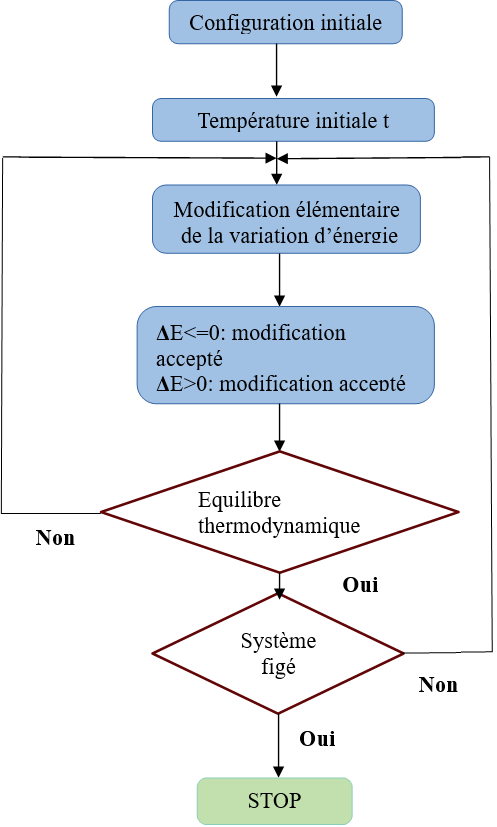
\includegraphics[width=9cm,height=10cm]{Chap2/3.png}
	\caption{Organigramme  illustrant le fonctionnement  de la recherche Recuit simulé}
	\label{fig:OIFRR}
\end{figure}

\begin{algorithm}[H]
\caption{Recuit simulé }
%\KwData{this text}
%\KwResult{la meilleure combinaison ayant appartenu à la population }
\SetAlgoLined
\DontPrintSemicolon
$ t \gets 0 $ , Initialiser la température T en fonction du schéma de refroidissement \;
$ s\gets s_0 $ , une solution initiale \;
$ Best \gets S $ \;
\While{(Best est la meilleure) $\cap$ (nombre iter=max) $\cap$ ($ t \leq 0 $)}{
  $ r \gets s’$ où $s’ \in N(s)$ \;
  $ \rho \gets random(0.1)$ \;
  $ \triangle E = f(r)-f(s) $  \;
  \If{ $ f(r) < f(s)  \cup \rho < e^{-\triangle E/t }$ }{
	$ s \gets r $ \;
   }
  \If{f(s)<f(Best)}{
	$ Best \gets s$ \;
   }
   Décrémenter le t \;
 }
\end{algorithm}


	\item \textbf{Recherche tabou: } La méthode de recherche avec tabous, ou simplement recherche tabou (TS :Tabu Search) a été formalisée par Fred Glover en 1986 \cite{glover1986future} . Elle utilise explicitement l’historique de la recherche, à la fois pour échapper aux minimaux locaux et pour mettre en œuvre une stratégie d’exploration. Sa principale caractéristique est en effet basée sur  l’utilisation de mécanismes inspirés de la mémoire humaine. A l'inverse du recuit simulé qui génère de manière aléatoire une seule solution voisine s’ \( \in N(s) \) à chaque itération, la recherche tabou examine un échantillonnage de solutions de \( N(s) \) et retient la meilleure s’ même si s’ est plus mauvaise que s. La recherche tabou ne s'arrête donc pas au premier optimum trouvé.\\
La méthode TS utilise une liste tabou, qui mémorise les dernières solutions rencontrées (ou des caractéristiques de solutions) vers lesquelles il est interdit de se déplacer. Ce procédé simple de mémoire permet de choisir le meilleur voisin non tabou, même si celui-ci dégrade la fonction-objectif f. Cependant, dans certains cas, les interdictions occasionnées par la liste tabou peuvent être jugées trop radicales. En effet, on risque d’éliminer (en les rendant tabous), certains mouvements particulièrement utiles. Pour éviter cela, on incorpore dans l’algorithme un mécanisme d’aspiration
qui détermine des critères selon lesquels un mouvement, bien que tabou, peut quand même être
accepté, s’il permet d’obtenir une meilleure solution que toutes celles déjà parcourues.\\
La taille de la liste tabou contrôle la mémoire du processus de recherche. Pour favoriser l’intensification, il suffit de diminuer la taille de la liste tabou. En revanche, augmenter la taille de la liste tabou, forcera le processus de recherche à explorer des régions plus vastes, favorisant ainsi la diversification. La taille de la liste tabou peut être modifiée au cours de la recherche \cite{battiti1994reactive}.\\
Une autre amélioration intéressante de la TS est l’utilisation de structure de mémoire à moyen et à long terme afin d’approfondir les notions d’intensification et de diversification.\\
\begin{figure}[H]
	\centering
	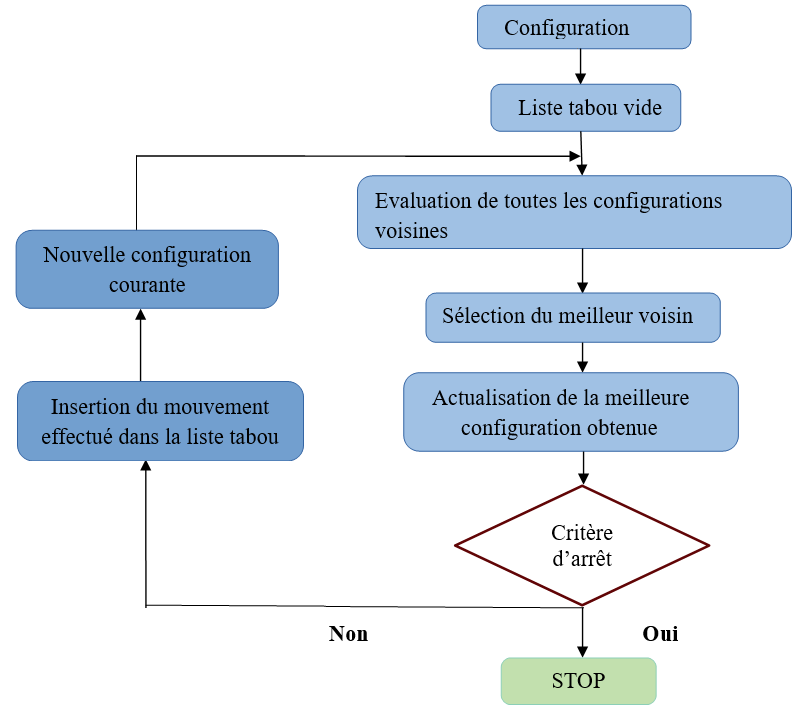
\includegraphics[width=12cm,height=8cm]{Chap2/4.png}
	\caption{Organigramme illustrant le  Fonctionnement de l’algorithme TS}
	\label{fig:OIFA}
\end{figure}
\begin{algorithm}[h!]
\caption{Recherche Taboue}
\SetAlgoLined
\DontPrintSemicolon
$ l \gets longueur maximale de la liste taboue $  \;
$ n \gets number of tweaks desired to sample the gradient$ \;
$ S \gets solution initial $ \;
$ Best \gets S $ \;
$ L \gets \{\} $ \;
Insérer s dans L \;

\While{(Best est la meilleure) $\cap$ (nombre iter=max)}{
  \If{ $ longueur(L) > l $ }{
    Défiler un élément de la liste L \;
   }
   $r \gets r’$ où  $r’ \in N(s)$  \;  
   \For{$i\gets1$ \KwTo $N-1$ }{
     $w \gets w’$ où  $w’ \in N(s)$  \;
     \If{$ w \notin L  \cap ( f(w)<f(r) \cup r \in L ) $ }{
		$ e \gets w $ \;
		\If{$ r \notin L  \cap f(r)<f(s) $}{
           $ s \gets r $ \;
           Enfiler r dans L \;
		}
		\If{$f(s)<f(Best)$}{
			$ Best \gets s $			
		}
     }
   }
 }

\end{algorithm}



	
	\item \textbf{Recherche locale : } Pour cette méthode de recherche il suffit de tester itérativement de nouvelles solutions potentielles dans la région de la solution courante, et de prendre la meilleure dans le voisinage. La méthode est une généralisation de la méthode de la descente de gradient elle consiste à partir d’une solution s à choisir une solution s’ dans un voisinage de s, noté N(s). La nouvelle solution choisie est meilleure que la précédente sous la fonction objective. Cela nous permet d’explorer l’espace des combinaisons  de proche en proche, en partant d’une combinaison initiale et en sélectionnant à chaque itération une combinaison voisine de la combinaison courante, obtenue en lui appliquant une transformation élémentaire jusqu’à la convergence à un optimum local. L’algorithme  décrivant le principe général de la recherche locale:\\

\begin{algorithm}[H]
\caption{Recherche Local}
\SetAlgoLined
\DontPrintSemicolon

$ s \gets solution initial $ \;
\While{ (Best est la meilleure) $\cap$ (nombre iter=max) }{
	$ r \gets s’$ où $s’ \in N(s)$ \;
	\If{ $f(r) < f(s)$ }{
		$ s \gets r $  \;		
	}
}

\end{algorithm}
	
	
	\item \textbf{Recherche à voisinages variables(VNS):} La recherche à voisinage variable (VNS : Variable neighborhood search) est une méta-heuristique proposée par Hansen et Mladenovic en 1997 [28,29]. Elle est basée sur le principe de changement systématique de voisinage durant la recherche (la performance des méthodes de descente).  La procédure de VNS se compose de trois étapes : perturbation (shaking), recherche locale et déplacement. Cet algorithme est efficace si les structures de voisinage sont complémentaires en ce sens qu’un minimum local pour un voisinage n’en n’est pas nécessairement un pour un autre, ce qui veut dire simplement d’utiliser plusieurs voisinages successifs quand on se trouve bloqué dans un minimum local.\\
	
\begin{algorithm}[H]
\caption{Recherche à voisinages variables (VNS)}
\SetAlgoLined
\DontPrintSemicolon

$ s \gets solution initial $ \;
\Repeat{$ K = K_{Max} $}{
	générer $s’$ ,tel que $s’ \in N(s)$ \;
	$s'' \gets Appel$(Recherche Locale) \;
	\eIf{$f(s'') < f(s)$}{
		$ s \gets s'' $ \;
		$ K \gets 1 $ \;		
	}{
		$ K = K + 1 $ \;
	}
}
	

\end{algorithm}

	
\end{enumerate}



\subsubsection{Méthodes évolutives (A population):}
Depuis le début des années 90, une autre famille d’ heuristiques est devenue très populaire : les Méthodes Évolutives \cite{hertz2000framework} , s’inspirant de la théorie de l’évolution «darwinienne»  tels que le croisement, la mutation et la sélection pour résoudre des problèmes divers. Contrairement à la Recherche Locale qui tente d’ améliorer itérativement une solution courante. Les Méthodes Évolutives travaillent sur une population de solutions en appliquant un processus cyclique composé d’ une phase de coopération et d’ une phase d’adaptation individuelle qui se succèdent à tour de rôle. Dans la phase de coopération, les solutions de la population courante sont comparées entre elles, puis combinées, dans le but de produire de nouvelles solutions qui héritent des bons aspects de chaque membre de la population. Dans la phase d’adaptation individuelle, chaque solution dans la population peut évoluer de manière indépendante. On peut utiliser le même type de critère d’ arrêt que dans la Recherche Locale, ou alors on peut décider de stopper une Méthode Évolutive dès que les solutions dans la population sont jugées trop similaires. Une description générale des Méthodes Évolutives est donnée ci-dessous:

\begin{figure}[H]
	\centering
	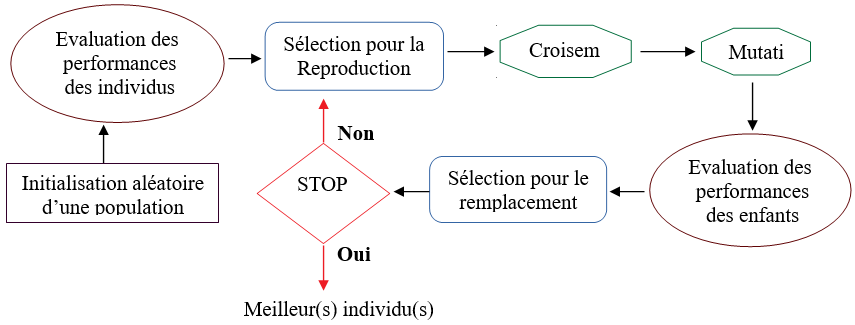
\includegraphics[width=15cm,height=7cm]{Chap2/5.png}
	\caption{Principe d’un algorithme évolutionnaire (EA) \cite{dreo2003metaheuristiques}.}
	\label{fig:PAEEA}
\end{figure}

Le terme Evolutionary Computation englobe une classe assez large de méta-heuristiques qui ont été développés au début des années soixante, telles que les algorithmes génétiques \cite{holland1975adaptation}, les stratégies d’évolution \cite{rechenberg1973evolutionsstrategie} , la programmation évolutive \cite{fogel1966artificial}, et la programmation génétique \cite{koza1992genetic}

\begin{enumerate}[label=\alph*)]
	\item \textbf{Algorithmes génétiques(AG):} développées par J. Holland en 1975 \cite{holland1975adaptation} comme outils de modélisation de l’adaptation et qui travaillent dans un espace de chaînes de bits. Elles ont été largement utilisé et développé par [ Moscato en 1989 \cite{moscato1989evolution} ]. Cette classe s’inspire de la théorie de l’évolution et des règles de la génétique qui expliquent la capacité des espèces de s’adapter à leurs environnement à l’ aide de l’ opérateur de mutation, alors que l’ échange d’information est gouverné par un opérateur de reproduction et un opérateur de combinaison (ou croisement). L’algorithme ci-dessous décrit ce principe général, dont les principales étapes sont détaillées ci-après.\\

\begin{figure}[H]
	\centering
	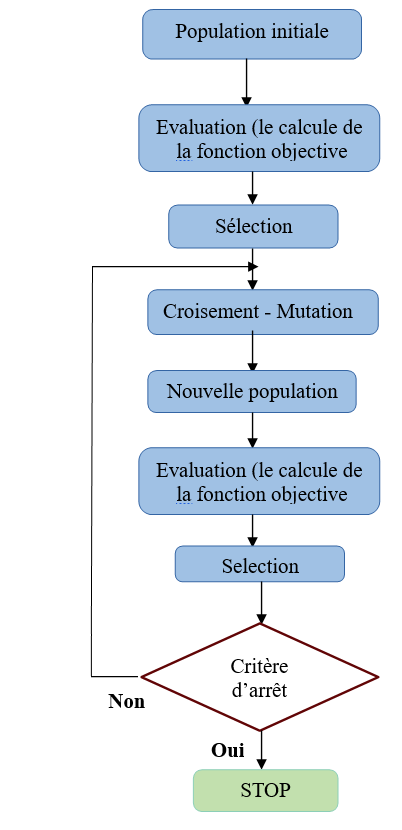
\includegraphics[width=9cm,height=10cm]{Chap2/6.png}
	\caption{Organigramme d’un algorithme génétique}
	\label{fig:OAG}
\end{figure}

\begin{algorithm}[H]
\caption{Algorithme génétique}
\KwResult{la meilleure combinaison ayant appartenu à la population }
\SetAlgoLined
\DontPrintSemicolon

Initialiser la population avec un ensemble de combinaisons de E \;
\While{critères d’arrêt non atteints}{
	Sélectionner des combinaisons de la population \;
	Créer de nouvelles combinaisons par croisement et mutation \;
	Mettre à jour la population  \;
}

\end{algorithm}

	
\begin{itemize}
	\item \textbf{Initialisation de la population: }en général, la population initiale est générée de façon aléatoire, selon une distribution uniforme assurant une bonne diversité des combinaisons. Une solution initiale est de bonne qualité, celle qui nous permet de converger vers un optimum global dans le plus court délai possible.\\
  Il est à noter que cette méthode est utilisée dans toutes les méta-heuristiques avec population.

	\item \textbf{Sélection: } cette étape consiste à choisir les combinaisons de la population qui seront ensuite croisées et mutées. Il s’agit là de favoriser la sélection des meilleures combinaisons, tout en laissant une petite chance aux moins bonnes combinaisons. Il existe de nombreuses façons de procéder à cette étape de sélection. Par exemple, la sélection par tournoi consiste à choisir aléatoirement deux combinaisons et à sélectionner la meilleure des deux (ou bien à sélectionner une des deux selon une probabilité dépendant de la fonction objectif).
	
	\item \textbf{Croisement:} est une opération de diversification. cette opération consiste à générer de nouvelles combinaisons, à partir des deux individus sélectionnés. Là encore, il existe de nombreux opérateurs de croisement. Une méthode simple consiste à choisir aléatoirement un point de croisement, à couper chaque combinaison parente en ce point, puis à reformer deux enfants en échangeant les parties composant les parents de part et d’autre du point de croisement.
	
	\item \textbf{Mutation: } cette opération consiste à modifier de façon aléatoire certains composants des combinaisons obtenues par croisement.
	
	\item \textbf{Mise à jour de la population: } cette étape consiste à remplacer certaines combinaisons de la génération précédente par certaines combinaisons issues des opérations de croisement et de mutation, formant de la sorte une nouvelle génération. Là encore, il existe différentes stratégies de remplacement, favorisant plus ou moins la diversité, et plus ou moins élitistes. On peut par exemple choisir de ne garder que les meilleurs individus, qu’ils soient issus de la nouvelle génération ou de l’ancienne, ou bien ne garder que les individus de la nouvelle génération, indépendamment de leur qualité.
	
	\item \textbf{Critères d’arrêt: } le processus d’évolution est itéré, de génération en génération, jusqu’à ce qu’une combinaison de qualité suffisante soit générée, ou bien jusqu’à ce qu’une limite de temps soit atteinte. On peut également utiliser des indicateurs de diversité (comme par exemple le taux de ré-échantillonnage ou la distance pair-à-pair) pour arrêter le processus lorsque la population est devenue trop uniforme. On peut aussi limiter le nombre d’itération possible ou encore les probabilités d’application des opérateurs de croisement et de 
mutation.
 
\end{itemize}	

	
	\item \textbf{L’optimisation des colonies de fourmis (ACO): }est une technique d’intelligence artificielle qui s'inspire du comportement intelligent des fourmis lors de la recherche de nourriture. Cette méta-heuristique permet de trouver des solutions de haute qualité aux problèmes d’optimisation combinatoire. 

En raison de leur comportement de recherche de nourriture, les fourmis trouvent les chemins les plus courts entre leur nid et leur source de nourriture, en déposant sur la terre une substance chimique appelée phéromone. Cela forme une traînée de phéromone qui est utilisée pour la communication stigmergique. La présence d'une telle phéromone sur les trajectoires affecte la prise de décision des fourmis concernant les trajectoires choisies par elles. Les fourmis sélectionnent de manière probabiliste les chemins marqués par de fortes concentrations de phéromones ce qui permet aux fourmis de trouver le chemin le plus court vers la source de nourriture.\\


\begin{algorithm}[H]
\caption{L’optimisation des colonies de fourmis (ACO)}
\KwResult{la meilleure solution trouvée}
\SetAlgoLined
\DontPrintSemicolon

\tcp{Initialisation}
initialisation de phéromones et les paramètre avec des valeurs constantes \;
Construction de la solution initiale \;
\While{condition d’arrêt non atteinte }{
	\While{nombre de fourmis non atteint}{
		Construction d’une solution selon la concentration de phéromone \;
		Mise à jour en ligne de  la table des phéromones \;
	}
	\If{la meilleure solution trouvée par l’itération courante est meilleure que celles des 	itérations précédente}{
		Mise à jour de l a solution courante \;
	}
	Mise à jour hors ligne de  la table des phéromones \;	
}

\end{algorithm}

\begin{itemize}
	\item \textbf{Solution initiale:} en général, la solution initiale est générée de façon aléatoire.Une solution est composée de plusieurs attributs définis selon la nature du problème.
	
	\item \textbf{Initialisation de la table de phéromone:} la table de phéromone contient  la concentration de phéromone pour tous les attributs possible d’une solution. Au départ tous les attributs ont une même concentration de phéromone. 
	
	\item \textbf{Mise à jour de phéromone:}
		\begin{itemize}
			\item \textbf{En ligne:} les attributs communs entre la solution courante et la meilleure solution vont être favoriser par une valeur constante supplémentaire.
			\item \textbf{Hors ligne:} les attributs appartenant à la meilleure solution vont être favoriser par la valeur constante. 
		\end{itemize}
\end{itemize}
	
	\item \textbf{L’algorithme à base de biogéographie (BBO)} BBO est un algorithme inspiré de la biogéographie, qui étudie la répartition géographique des organismes biologiques.

Tout comme GA et PSO qui sont basés sur la biologie, BBO est un algorithme basé sur une population dans lequel chaque population de solutions candidates est utilisée dans la procédure de recherche d’un optima global. BBO présente certaines caractéristiques communes avec l’algorithme d'optimisation, le GA. En GA, un individu de la population s'appelle un chromosome et a sa propre valeur de condition physique. De même, dans BBO, chaque individu est qualifié d'habitat et a son indice de qualité de l'habitat (HSI) pour évaluer sa qualité en tant que solution. Comme nous avons affaire à un problème de minimisation, un habitat à faible indice de sécurité d'impact représente une bonne solution et un habitat à haut indice de faiblesse est plutôt une solution médiocre. Chaque chromosome de GA est constitué de gènes, tandis que, pour BBO, chaque habitat est caractérisé par des variables d'indice de pertinence (SIV). L'AG compte deux opérateurs principaux: le croisement et la mutation. Pendant ce temps, chez BBO, les principaux opérateurs sont la migration et la mutation. L'opérateur de migration est composé d'émigration et d'immigration. Il est utilisé pour améliorer et faire évoluer les habitats (solutions au problème d'optimisation) de la population. Les fonctionnalités de solution (SIV) émigrent d'habitats à faible HSI (habitats d'émigration) vers des habitats à haut HSI (habitats d'immigration). Il existe différentes alternatives pour les processus de migration et de mutation de BBO. La manière dont nous implémentons ces deux opérateurs est expliquée en détail dans le prochain chapitre. \\


\begin{algorithm}[H]
\caption{L’algorithme à base de biogéographie (BBO)}
\KwResult{la meilleure solution ayant appartenu à la population }
\SetAlgoLined
\DontPrintSemicolon

Générer aléatoirement un ensemble de solutions initiales (îles) \;
\While{le critère d’arrêt n’est pas atteint}{
	Évaluer la fitness (HSI) de chaque solution \;
	Calculer le nombre d’espèce $S$, le taux d’immigration $\lambda$ et d’émigration $\mu$ pour chaque solution \;
	\textbf{Migration}  \;
	\textbf{Mutation} : muter les individus au taux de mutation \;
	Remplacement de la population par les descendants \;
	Implémenter l’\textbf{élitisme}  \;
}

\end{algorithm}

Dans le processus de migration (algorithme \ref{alg:MIGRATION}), quand une solution est sélectionnée pour être changée, nous utilisons le taux d'immigration $\lambda$ pour décider si un SIV sera changé. Dans ce cas, nous utilisons le taux d'émigration $\mu$ pour décider quelle bonne solution migrera son SIV.\\
Cette algorithme  sera suivit d’une figure qui ellustre le fonctionnement de ce processus (figure \ref{fig:PMBBO}) \\

\begin{algorithm}[H]
\label{alg:MIGRATION}
\caption{migration}
\SetAlgoLined
\DontPrintSemicolon

\For{$i\gets1$ \KwTo $N$}{
	Utiliser $\lambda_i$ pour décider, de manière probabiliste, d’immigrer à $X_i$ \;
	\If{$rand(0,1) < \lambda_i $}{
		\For{$j \gets 1$ \KwTo $N$}{
			Sélectionner un habitat d’émigration $X_j$ avec une probabilité $\alpha \mu_j $ \;
			\If{$rand(0,1) < \mu_j$}{
				Remplacer une variable de décision (SIV) choisie aléatoirement dans par la variable correspondante dans $X_j$ \;				
			}
		}
	}
}

\end{algorithm}



Où : \\
$\lambda_k$ : est le taux d'immigration dans un habitat de k espèces \\
$\mu_k $ : est le taux d'émigration dans un habitat de k espèces. \\
$E$ : est le taux maximal d'émigration.\\
$I$ : est le taux maximal d'immigration. Supposons que nous avons une population de solutions candidates à un problème, représentées par des vecteurs (habitats $H_i , i = 1...n $)\\
$N$ : est le nombre maximum d'espèces.\\
$k$ : est le nombre d'espèces.\\
\textbf{Mutation:} c’est le même principe qui est utilié pour l’algorithme génétique.\\
\textbf{Elitisme:} cette méthode consiste à garder les meilleurs individus de chaque population. La méthode d’élitisme risque d’élaguer les individus de mauvaise qualité mais ça n’empêche pas de produire une population avec des résultats meilleurs ou au moins de créer des individus qui auront pu apporter de quoi créer de très bonnes solution dans les populations suivantes. \\

\begin{figure}[H]
	\centering
	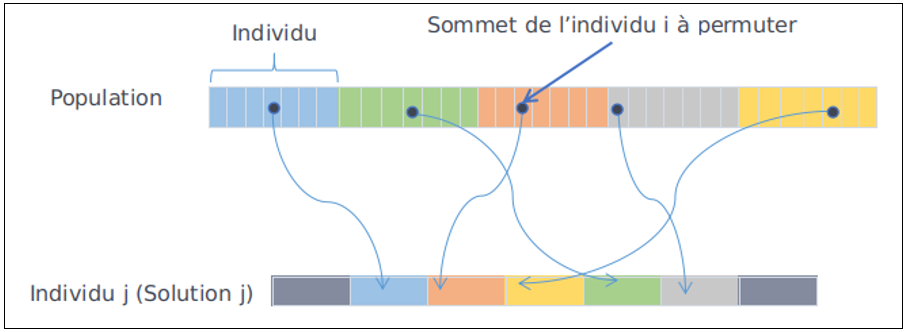
\includegraphics[width=15cm,height=6cm]{Chap2/7.png}
	\caption{processus de migration de BBO}
	\label{fig:PMBBO}
\end{figure}	
	
	\item \textbf{Algorithmes mémétiques (algorithme de colonies de fourmis \& d’essaim de particules) : }
Le terme «algorithmes mémétiques»  est apparu pour la première fois dans [38], introduit par Moscato en 1986. L’idée principale de ce genre d’algorithme est de rendre plus agressif un algorithme génétique par l’ajout d’une recherche locale en plus de la mutation.

La faible vitesse de convergence est la première observation provenant de l’implémentation de l’algorithme génétique. Pour cet effet Moscoto a pensé d’ajouter une recherche locale  qui peut être une méthode de descente ou une recherche locale plus évoluée (recuit simulé ou recherche tabou par exemple). Cette recherche locale sera appliquée à tout nouvel individu obtenu au cours de la recherche.

D’une vue globale, l’application de cette simple modification n’influe en rien sur le comportement de l’algorithme, mais  cela peut apporter de profondes changement en ce dernier. Après avoir créé un nouvel individu à partir de deux parents sélectionnés, on applique une recherche locale et sous certaines conditions on applique un opérateur de mutation à cet individu. Les conditions peuvent être une certaine probabilité. Il est aussi possible d’ajouter un critère d’aspiration ou d’autres techniques plus évoluées à cet endroit.\\


\begin{algorithm}[H]
\caption{Simple Algorithme mémétique}
\KwResult{la meilleure solution ayant appartenu à la population }
\SetAlgoLined
\DontPrintSemicolon

Initialisation : générer une population initiale $P$ de solutions de taille $| P | = n$  \;
\Repeat{critère d'arrêt satisfait}{
	Sélection: choisissez 2 solutions s et $s’$ avec la technique volue \;
	Croisement: combinez les solutions parentes s et $s’$ pour former une solution enfant $y$ \;
	Recherche locale: appliquer une procédure de recherche locale sur y sous certaines conditions \;
	Mutation: appliquer un opérateur de mutation sur y dans des conditions \;
	Choisir un individu y’ à remplacer dans la population \;
	remplacer y’ par y dans la population \;	
}

\end{algorithm}

\begin{figure}[H]
	\centering
	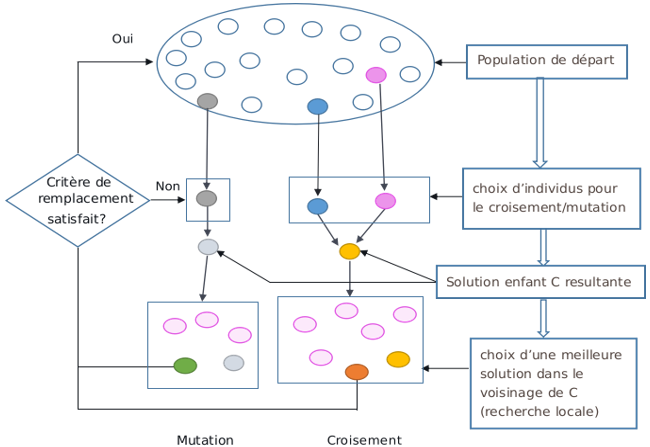
\includegraphics[width=15cm,height=10cm]{Chap2/8.png}
	\caption{Schéma explicatif d’un algorithme mémétique}
	\label{fig:SEAM}
\end{figure}
	
\end{enumerate}


\section{Conclusion}
Nous avons présenté dans ce chapitre l’état de l’art des méta-heuristiques pour l’optimisation des problèmes Np-difficile. Plus de détails sur le problème de l’arbre dominant qui en est un, ainsi que les méthodes utilisées pour sa résolution seront mis au clair dans le prochain chapitre.

